\begin{frame}{Time for a history lesson...}
   The historical derivation of DFT+\emph{U}: let's integrate the Hubbard model into the DFT framework!
   \vspace{6pt}

   \onslide<2->{
      Start with an electron-electron interaction term...
      %
      \begin{equation*}
         \hat U = \sum_{mnm'n'}\sum_{\sigma\sigma'}U_{mnm'n'}c^\dag_{m\sigma} c^\dag_{n\sigma'} c_{m'\sigma'} c_{n'\sigma},
      \end{equation*}
   }
   \onslide<3->{We make various assumptions:
   \begin{itemize}
      \item ignore all but two-site interaction terms (\`a la Hubbard model)
      \item neglect terms between opposite spin (likewise)
      \item adopt a double-counting term % (fully localised limit, all subspaces with integer occupancy)
      \item assume single-Slater-determinant wavefunction
   \end{itemize}}

   \onslide<4->{
      ... and finish with a correction term to DFT
      %
      \begin{align*}
         E_{DFT+U}[\rho] = E_\mathsf{DFT}[\rho] + E_\mathsf{U}[\rho] = E_\mathsf{DFT}[\rho] + \sum_{I\sigma} \frac{U^I}{2}\Trace[\hat n^{I\sigma}(1-\hat n^{I\sigma})]
         \label{eqn:EU3}
      \end{align*}
   }
\end{frame}

\begin{frame}{Method 1: DFT+\emph{U}}
   The DFT\,+\,\emph{U} correction in detail:
   \begin{align*}
      E_\mathsf{U} = \sum_{I\sigma} \frac{U^I}{2}\Trace[\hat n^{I\sigma}(1-\hat n^{I\sigma})]
   \end{align*}
   %
   \begin{align*}
      \hat n^{I\sigma} = \hat P^I \hat \rho^\sigma \hat P^I = \sum_{i,j} \ket{\varphi^I_i}\bra{\varphi^I_i} \hat \rho^\sigma \ket{\varphi^I_j}\bra{\varphi^I_j}
   \end{align*}
   \begin{minipage}[t][0.5\paperheight][t]{\textwidth}
      \only<2>{
         \begin{center}
            \begin{tabular}{ccccc}
               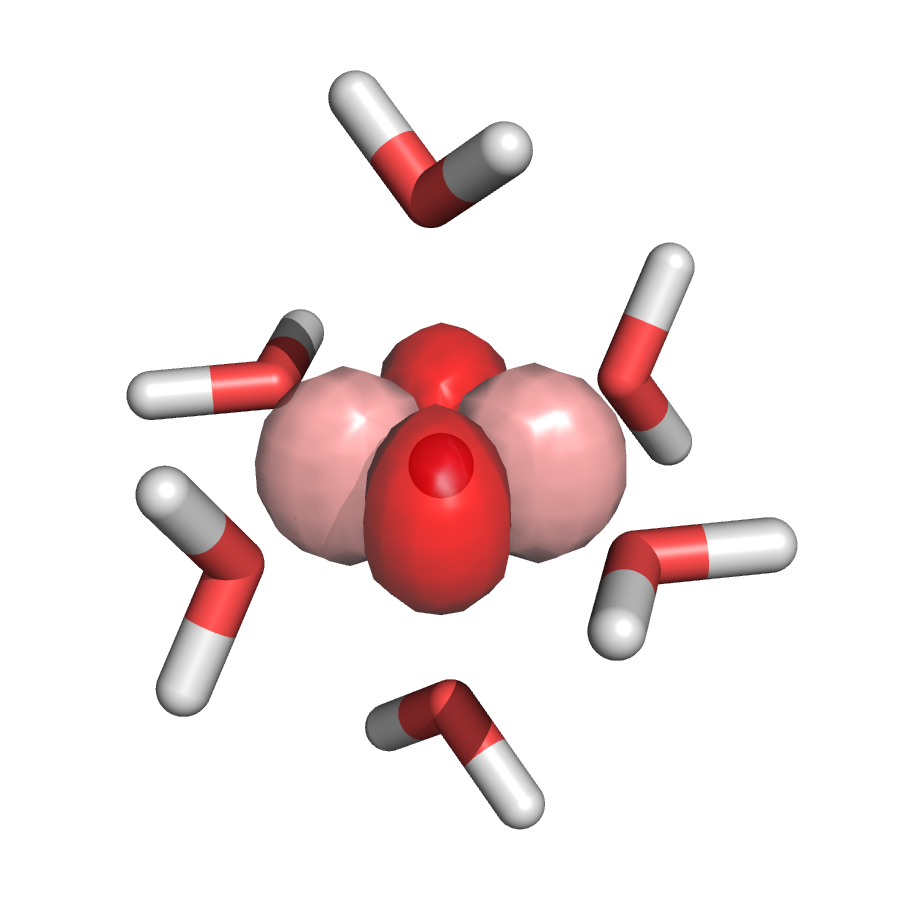
\includegraphics[trim=4cm 2cm 3cm 2cm, clip, width=0.16\textwidth]{figures/Mn3+_dxy.png} &
               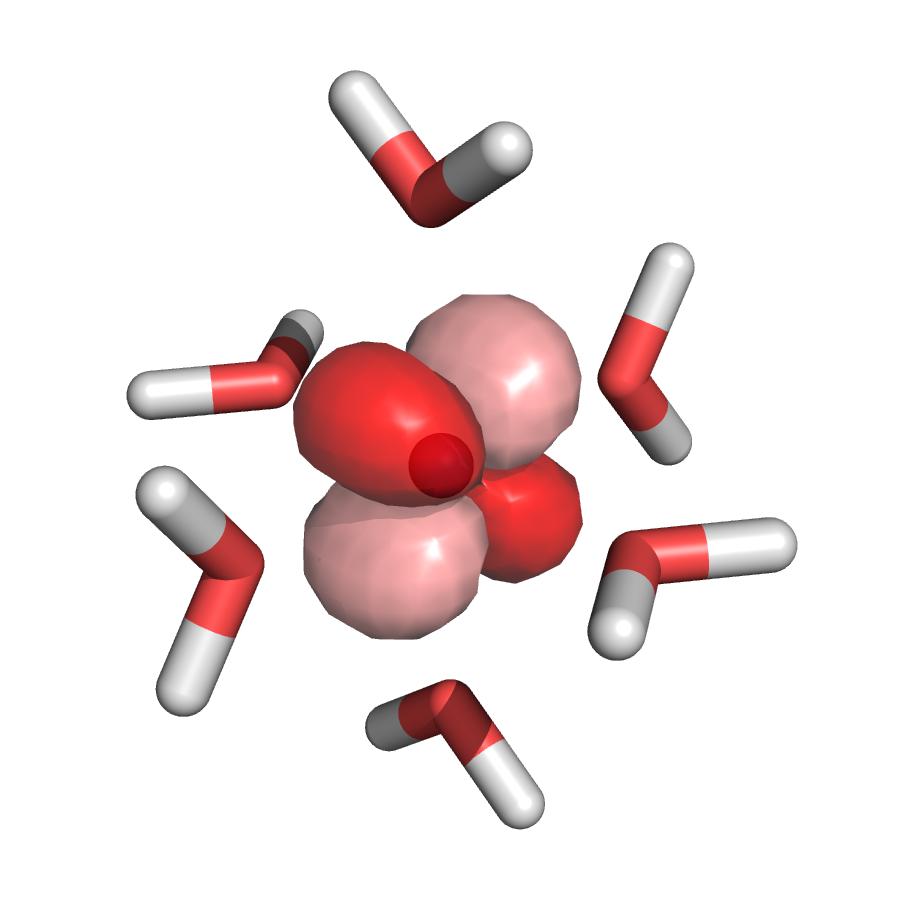
\includegraphics[trim=4cm 2cm 3cm 2cm, clip, width=0.16\textwidth]{figures/Mn3+_dxz.png} &
               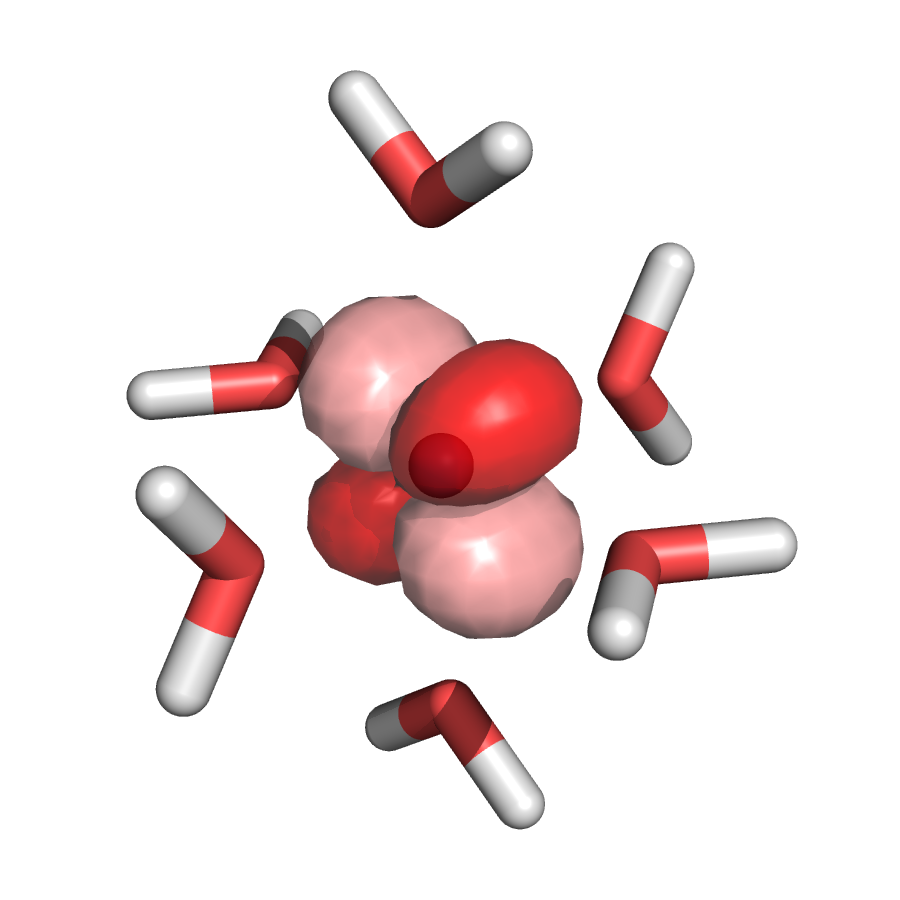
\includegraphics[trim=4cm 2cm 3cm 2cm, clip, width=0.16\textwidth]{figures/Mn3+_dyz.png} &
               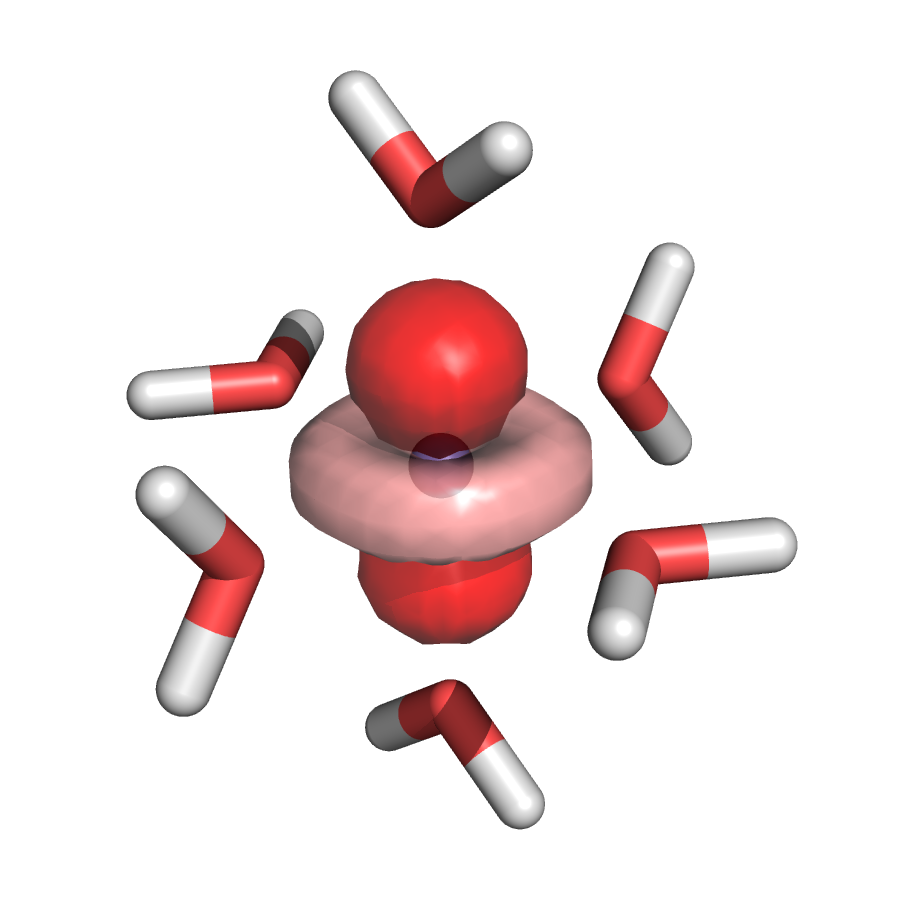
\includegraphics[trim=4cm 2cm 3cm 2cm, clip, width=0.16\textwidth]{figures/Mn3+_dz2.png} &
               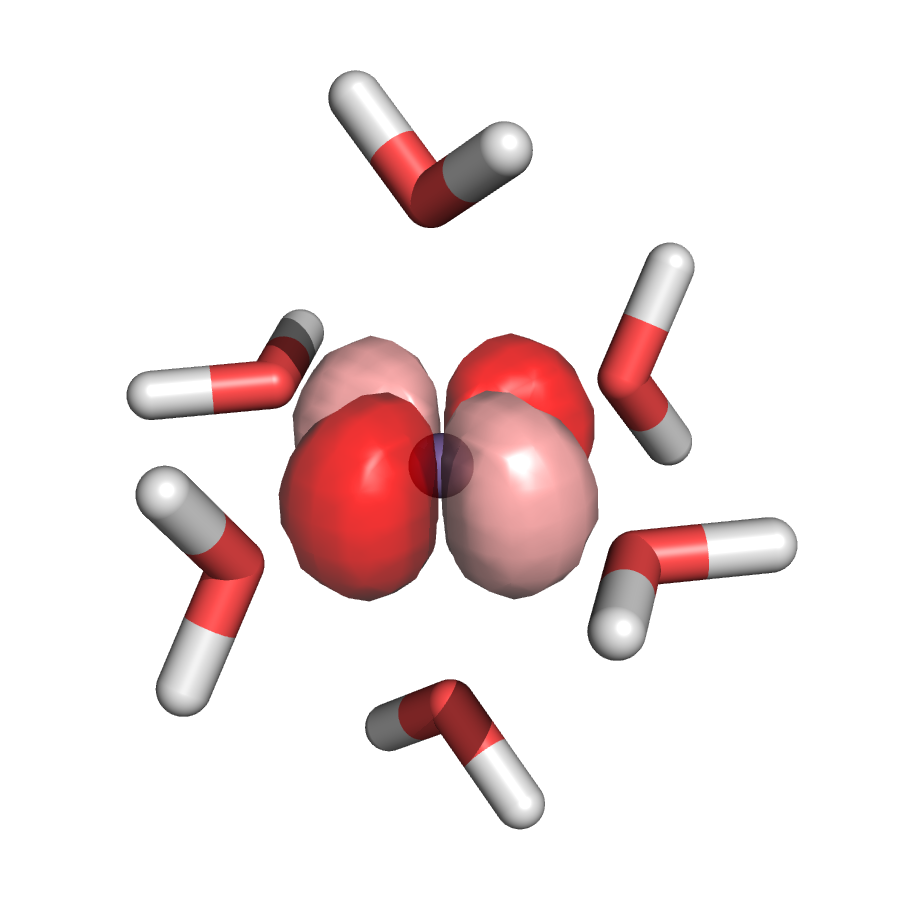
\includegraphics[trim=4cm 2cm 3cm 2cm, clip, width=0.16\textwidth]{figures/Mn3+_dx2-y2.png} \\
               $ \braket{\mathbf{r}}{\varphi^I_1} $ &
               $ \braket{\mathbf{r}}{\varphi^I_2} $ &
               $ \braket{\mathbf{r}}{\varphi^I_3} $ &
               $ \braket{\mathbf{r}}{\varphi^I_4} $ &
               $ \braket{\mathbf{r}}{\varphi^I_5} $
            \end{tabular}
         \end{center}
      }
      %
      \only<3>{
         \begin{align*}
            \hat V_\mathsf{U} = \sum_{I\sigma ij}U^{I} \ket{\varphi^I_i}\left(\frac{1}{2}-n_{ij}^{I\sigma} \right) \bra{\varphi^I_j}
         \end{align*}
         %
         Creates gap of $U$ between filled and empty states
      }
   \end{minipage}
\end{frame}

\begin{frame}{Method 1: DFT+\emph{U}}
   \vspace{-3ex}
   \begin{center}
      \only<1>{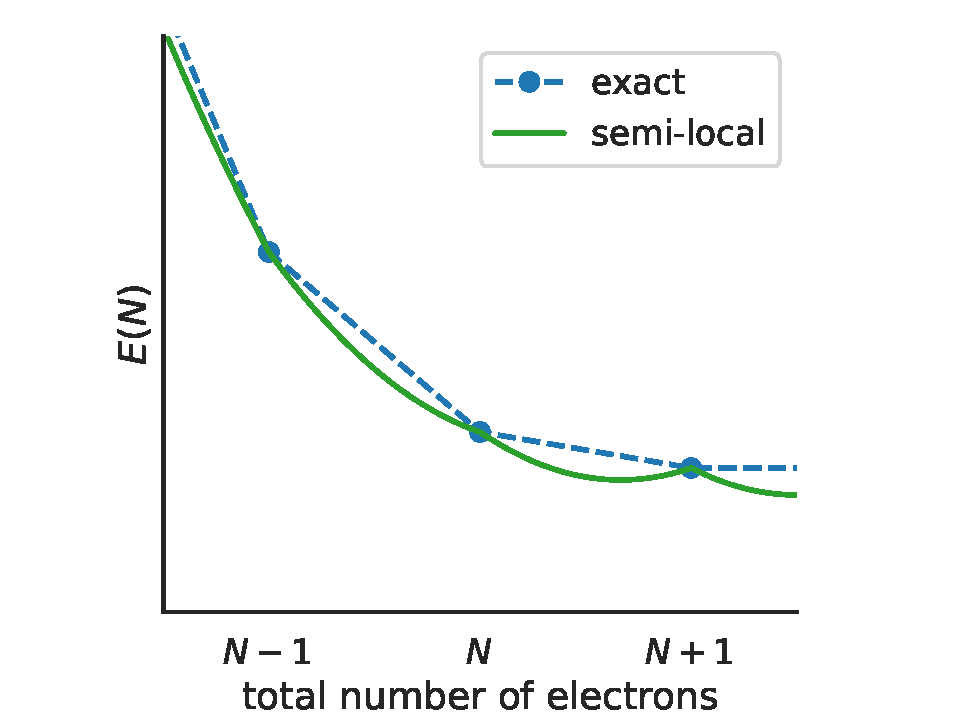
\includegraphics[height=0.5\textheight]{figures/curvature_plot/fig_en_curve_dftu_without_correction.pdf}}
      \only<2->{
      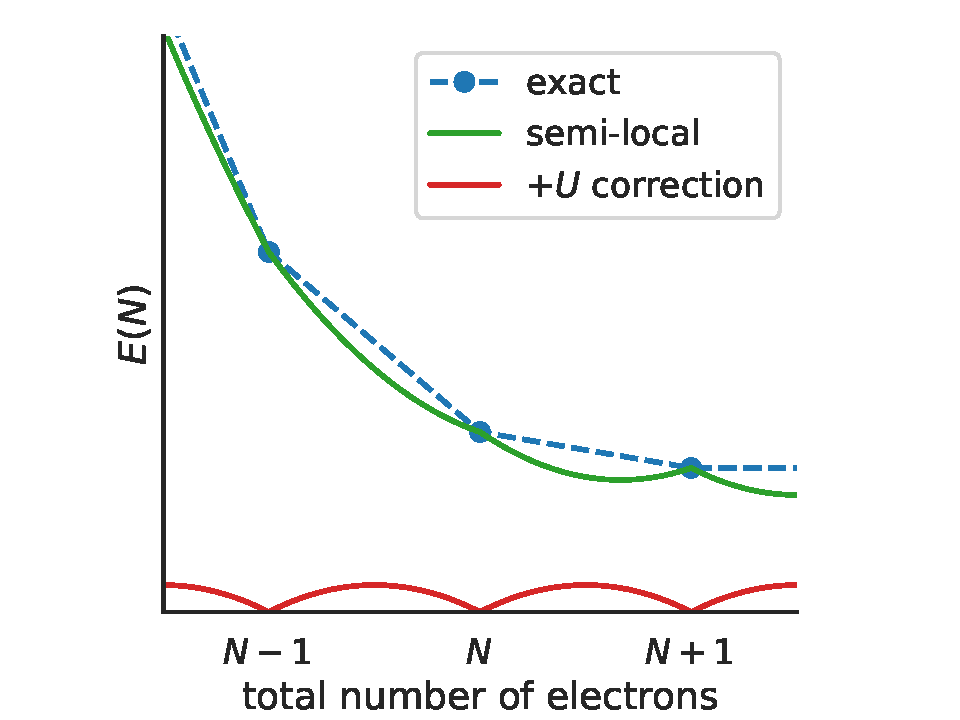
\includegraphics[height=0.5\textheight]{figures/curvature_plot/fig_en_curve_dftu_correction.pdf}}
   \end{center}

   \small
   A modern interpretation:
   in a basis such that $\hat n^{I\sigma} =diag(\lambda^{I\sigma}_1, ... ,\lambda^{I\sigma}_n)$
   \begin{align*}
      E_\mathsf{U} = \sum_{I\sigma} \frac{U^I}{2}\Trace[\hat n^{I\sigma}(1-\hat n^{I\sigma})]
      = \sum_{I\sigma} \frac{U^I}{2}\sum_i \lambda^{I\sigma}_i (1-\lambda^{I\sigma}_i)
   \end{align*}
   % \begin{center}
   %    \onslide<3->{\includegraphics[height=0.4\paperheight]{../figures/fig_En_theory.pdf}} 
   % \end{center}
   \onslide<3->{We can calculate $U$ via linear response $\rightarrow$ ``self-correcting" DFT}
   \blfootcite{Cococcioni2005a}
\end{frame}